\documentclass[12pt,a4paper]{article}

%% Language and font encodings
\usepackage[utf8x]{inputenc}
\usepackage[T1]{fontenc}

%% Sets page size and margins
\usepackage[a4paper,top=2cm,bottom=2cm,left=3cm,right=3cm,marginparwidth=1.75cm]{geometry}

\usepackage[affil-it]{authblk} 

\setlength{\parindent}{0pt}
\setlength{\parskip}{\baselineskip}


%% Useful packages
\usepackage{amsmath}
\usepackage{graphicx}
\usepackage[colorinlistoftodos]{todonotes}
\usepackage[colorlinks=true, allcolors=blue]{hyperref}
\usepackage{mathptmx}
\usepackage{titlesec}
\usepackage{lipsum}
\usepackage{mathtools}
\DeclarePairedDelimiter\floor{\lfloor}{\rfloor}
%\usepackage[utf8x]{inputenc}
%\usepackage[T1]{fontenc}

\usepackage{lmodern}
\usepackage{verbatim}
\usepackage{listings}
\usepackage{array}
\usepackage{multirow}
\usepackage{booktabs}
\usepackage{longtable}
\usepackage{makecell}
\usepackage{microtype}%if unwanted, comment out or use option "draft"
\usepackage{amsthm}
\usepackage{indentfirst}
\usepackage{color}
\usepackage{xcolor}
\usepackage{mathtools}
\usepackage{tikz}
%\usepackage[nottoc]{tocbibind}
\PassOptionsToPackage{greek,english}{babel}
\usepackage{apacite}
%\usepackage[english]{babel}
\usepackage{natbib}

%\usepackage{microtype}%if unwanted, comment out or use option "draft"
%\usepackage{fancyhdr,graphicx,amsmath,amssymb}
%\usepackage{mnsymbol}

\usepackage{algorithm}
\usepackage{algpseudocode}
\usepackage{amsthm}
\usepackage{indentfirst}
\usepackage{color}
\usepackage{xcolor}
\usepackage{mathtools}
\usepackage{lscape} %para poner la hoja de una tabla posicion horizontal
\usepackage{rotating}

\usepackage{smartdiagram}
\usesmartdiagramlibrary{additions}
\usepackage{newfloat}
\usepackage{caption}

\usepackage{xfrac} %permite hace fracciones con linea en diagonal

\DeclareFloatingEnvironment[fileext=diag,placement={!ht},name=Diagram]{diag}

\usepackage{tikz}
\usetikzlibrary{decorations.pathreplacing,automata,arrows,shadows,patterns}



%% Set headings 
\renewcommand\Authfont{\fontsize{12pt}{14.4pt}\selectfont}
\renewcommand\Affilfont{\fontsize{10pt}{10.8pt}\selectfont}

\titleformat{\section}
  {\normalfont\fontsize{12}{15}\bfseries}{\thesection.}{1em}{}
\titleformat{\subsection}
  {\normalfont\fontsize{12}{15}\bfseries}{\thesubsection}{1em}{}
  

\titlespacing*{\section}
  {0pt}{1\baselineskip}{0\baselineskip}
\titlespacing*{\subsection}
  {0pt}{0\baselineskip}{0\baselineskip}

\usepackage{caption}

\captionsetup{font=bf}

\usepackage{apacite}
\usepackage[english]{babel}


\addto{\captionsenglish}{%
    \renewcommand{\refname}{REFERENCES}}
\title{\bfseries \normalsize Assessing feasible approaches for building the consideration set in public transport route choice modeling using smart card data}


\author[1]{Jacqueline Arriagada*}
\author[2]{C. Angelo Guevara}
\author[3]{Marcela A. Munizaga}

\affil[1]{Departamento de Ingenier\'ia Civil Industrial, Universidad de Chile, Santiago, Chile.}
\affil[2,3]{Departamento de Ingenier\'ia Civil, Universidad de Chile, Santiago, Chile}
\affil[2,3]{Instituto Sistemas Complejos de Ingenier\'ia (ISCI)}
%\address{$^1$ Academic title, Department, University, Country \\ $^2$ Job position, Company, Country}

\date{\vspace{-5ex}}
%\affil[$\dagger$]{Department of Mathematics, Pennsylvania State University,Pittsburgh, Pennsylvania 13593}




\begin{document}
\maketitle
\section*{Abstract}
%% Text of abstract
\small
Choice modeling requires the researcher to know the consideration set (the group of alternatives that the individual considers when making a choice), but that almost never occurs. Various feasible approaches had been proposed for this but, so far, no comprehensive assessment of these approaches has been possible. This study contributes to close this gap by proposing and applying a methodology to assess seven feasible approaches to address the consideration set problem in public transport route choice models, both from a theoretical perspective and using four weeks of revealed preferences constructed from smart card data from Santiago, Chile. The approaches under study are K-shortest paths, Labeling, Link elimination, Link penalty, Simulation, Combined (mix of all previous approaches), and the Historical/Cohort method. The first six methods emulate heuristics that individuals may use for building the consideration set, while the seventh is originally based on intuition but can also be fully justified from a theoretical viewpoint by reinterpreting the theorem of estimation and sampling of alternatives. For the empirical assessment, the first three weeks of smart card data are used for estimation and to assess the fit and behavioral coherence attained with the feasible approaches under study. We use two specifications, the multinomial logit model and the path size logit model, to account for the correlation of routes. The fourth week of data is used for out-of-sample prediction analysis. The methods under study are also contrasted in terms of three coverage indicators for estimation and forecasting. The analysis shows that the Historical/Cohort method outperforms all other feasible approaches analyzed in all measures considered. This strong empirical evidence supporting the Historical/Cohort approach is in line with the theoretical results supporting it and suggests the convenience of using this approach, whenever feasible, beyond the public transport route choice context. However, theoretical and practical challenges remain to be addressed, especially regarding its applicability in forecasting.

\textbf{Keywords}: public transport, route choice, smart card data, passenger behavior.

\chapter{}\label{c3}


\section{Introduction}

To properly estimate and forecast with discrete choice models, it is crucial to identify the set of alternatives that were truly considered by an individual when making a choice. The problem is exacerbated when the number of alternatives is excessively large, as is the case in route choice models, but it is always an issue in any choice situation. The composition of the consideration set assumed by the researcher may importantly impact the model estimates and the predicted choice probabilities \citep{bliemer2008impact,prato2007modeling}, since a wrong assumption implies a potentially severe misspecification. Although  various feasible approaches have been proposed to build consideration sets for route choice modelling, to date, no comprehensive assessment of these approaches has been possible because of data and methodological limitations. Furthermore, little is known about the impacts of the composition of the consideration set in the case of public transport route choice modeling. This study contributes to close this gap by proposing and applying a methodology to assess seven feasible approaches to address the consideration set problem in public transport route choice models, using four weeks of revealed preferences constructed from smart card data from Santiago, Chile.

The methods proposed to address the consideration set problem can be broadly classified in two categories. The first uses a single-stage approach to model the consideration and the choice, while the second uses a two-stage approach. In the first category, all available alternatives are implicitly considered in the utility function, but some alternatives are penalized when attributes violate certain parameters, up to a point in which they cannot be chosen \citep{castro2013estimation, martinez2009constrained}. These methods require identifying all possible alternatives, which is feasible in scenarios with a small number of optionschoices, but becomes infeasible for larger choice-sets, such as those involved in route choice modeling . Because of this, and because evidence has shown that the consideration set and the choice from considered alternatives involve distinct mental processes, it has been suggested that it is preferable to explicitly model the consideration and the choice stages separately \citep{prato2009route}.

There is a vast literature that discusses the identification of the consideration set prior to the route choice model. Three types of literature within this realm can be distinguished. The first group corresponds to theoretical contributions related to discrete choice models that explicitly include the construction of the consideration set in their analysis. The seminal work in this regard corresponds to \cite{manski1977structure}, who proposes an approach where the consideration set is treated as a latent variable. Even though \cite{manski1977structure}’s approach theoretically solves the issue, in practical terms, it has two problems. The first is that is unclear how to appropriately define a practical function for the probability of considering a given latent set. The second is that the method involves enormous computing costs to enumerate all the combinations of possible consideration sets, an almost impossible task in the case of route choices in dense transit networks. To solve these practical problems, \cite{swait1987incorporating} and \cite{ben1995discrete} propose using individual characteristics (e.g., income or driver’s license ownership) or restrictions (e.g., distance) to develop expressions for the consideration-set probability, and to consider simplifying assumptions to reduce the number of potential latent sets. This approach, although intuitively appealing, is still an ad-hoc solution to the problem. Furthermore, although this approach may be feasible for choice-sets with a reduced number of alternatives, it quickly becomes infeasible for problems involving many options, such as route choice models.

A second group of studies separating the consideration set problem from the choice stage are empirical contributions, mainly in marketing, that investigate the size of the consideration set and the factors that may influence alternative consideration \citep{brown1992consideration, hauser2014consideration}. Similarly, in transportation, \cite{hoogendoorn2004multimodal} contrast the consideration set stated by the individual with an “objective set” that was built by first enumerating all feasible alternatives within a space-time window and then reducing the set using a branch and bound algorithm based on logical constraints. The authors conclude that, while the number of alternatives available to the travelers may be very large, the set of alternatives perceived is substantially smaller and even fewer alternatives are finally considered. In this regard, \cite{villalobos2018caracterizacion} show results that suggest that using stated preferences to collect information on the consideration set may be prone to severe hypothetical bias, reflected in the fact that the size of the consideration set gathered from such tools depends systematically on the experimental setting. 

A third group of studies, mainly focused on route choice modeling, aims to develop practical methods for generating the consideration set. A practical, or feasible, method is usually an algorithm or heuristic that tries to reproduce or emulate the behavior that individuals may follow when building their consideration set. Our research effort falls within this category, with an emphasis on the public transport  case, for which we have extensive revealed preferences observations constructed from smart card data.

The existing literature on public transport users’ route preferences has applied both stated preference (SP) data and revealed preference (RP) data. The studies that have used SP data \citep[e.g.][]{eluru2012travel, grison2017users, vrtic2002impact} obtain the information from a survey that asks people to choose a route from a set of alternatives in a hypothetical route choice situation, which may or may not be pivoted overbased on  a real trip situation. This methodology to obtain the data has the advantages of being relatively inexpensive and allowing the researcher to know the true consideration set faced by the respondent, but it introduces hypothetical bias, since the user does not experience an actual trip.

On the other hand, the use of RP data has the advantage of reflecting true information about the users’ choices in real situations, but, in this case, the researcher does not know the true consideration set, and data collection costs are higher. Public transport route choice studies that work with RP data may use traditional travel survey methods to capture choices and attributes, but these are not only expensive but also impractical for large samples \citep{guo2011mind,guo2011assessing, raveau2011topological, raveau2014behavioural, raveau2014analyzing, ton2020understanding, vrtic2002impact}. Recently, some authors have dealt with this problem using smart card data. The main purpose of smart cards is to collect public transport fares but, as a side benefit, they also collect a large quantity of very detailed data regarding the choices made by public transport users at significantly lower costs when compared with traditional survey methods, with few practical limitations, and with unprecedented granularity and scalability \citep{pelletier2011smart}.

In the context of public transport route choice studies that use RP data, the consideration set generation process is a complex task, since, usually, there are countless feasible alternative routes in a transport network, especially in a dense multimodal one. Two ways to identify the consideration set in practice can be distinguished in the applied literature: build it using an algorithm or heuristic that emulates how individuals may build the consideration set, or impute it from historical data. Most of the heuristics used to build feasible consideration sets in practice are based on iterating some type of deterministic shortest path \citep{prato2009route}. Some typical heuristic approaches are the K-shortest path, the Labeling \citep{ben1984modelling}, the Link elimination, the Link penalty, the Stochastic path methods, and a combination of previous methods. On the other hand, in the last decade to tackle the consideration set problem has been to impute it from historical data, i.e., previous choices made in a similar situation \citep{yap2020crowding, kim2019calibration, janovsikova2014estimation, raveau2011topological, raveau2014behavioural}. We denominate this method as the Historical/Cohort approach, which can be formally defined as building a practical consideration set from some collection of all observed choices made by the traveler in some timeframe prior to the instance under analysis, or the collection of observed choices of other users in the same cohort in cross-section data. Our research implements and assesses six typical heuristic approaches, together with the Historical/Cohort approach, which has become feasible with the advent of smart card data.

Beyond the consideration set problem, which is the focus of this research, another important challenge in public transport route choice modeling is the high level of correlation between route alternatives that share various links \citep[e.g.][]{prato2009route}, which alters the choice probabilities of overlapping routes. Therefore, route choice models must properly represent the correlation structure among alternative routes. Most studies of public transport passenger route choice behavior have used the Multinomial Logit (MNL) discrete choice model \citep{schmocker2013generation, nassir2018strategy, janovsikova2014estimation, kim2019calibration, grison2017users, guo2011mind, raveau2011topological, raveau2014behavioural, raveau2014analyzing, vrtic2002impact}, which assumes independence of alternatives, and therefore ignores the correlation problem due to overlapping route segments. To address this limitation, the analytical Path Size (PS) Logit approach has been proposed, which accounts for correlation by adding a deterministic term that reduces the utility of overlapped alternatives \citep{yap2020crowding, rui2016modeling, anderson2017multimodal, bovy2005modelling, de2012fixed, hoogendoorn2005path, nielsen2020relevance}. Our research implements both types of models, the basic MNL model and the PS Logit model.

In this article we assess the relative performance of seven feasible approaches to address the consideration set problem for public transport route choice modeling using revealed preferences data. The revealed preference data is built using three weeks of smart card transaction data, representing the actual route choice behavior of passengers who used Santiago, Chile’s dense public transport network. For the analysis, we use two specifications, the multinomial logit model and the path size logit model. We first evaluate the impact of different consideration set generation approaches by assessing the plausibility of the model estimates and the in-sample fit attained by each approach using different statistics and criteria. We conclude by studying the out-of-sample prediction performance attained by each method using the fourth week of data.

The remainder of this paper is organized as follows. Section 2 presents a formal demonstration of why the Historical/Cohort approach can be used to obtain consistent estimators of the model parameters. Section 3 describes the case study, the Santiago, Chile transit network. Section 4 discusses the proposed methods used for the consideration set and route choice models. Section 5 introduces the estimation and prediction results. Section 5 concludes and discusses policy and research implications.

\section{On The Theoretical support for feasible approaches to building the consideration set}

Despite the increasing sophistication of feasible approaches to building the consideration set, methods that are based on repeatedly varying some type of deterministic shortest path are just heuristics that attempt to emulate a supposed consideration behavior. There is no theoretical support for them beyond the assumption that the individual’s choices are rational, according to the researcher. Whenever the true consideration behavior varies from the rational behavior assumed by the researcher, the practical results may be poor. Therefore, empirical assessment of any of proposed method under a common framework is critical; however, it has been scarcely applied. \cite{villalobostesis2021} presented Monte Carlo evidence along these lines. In the next section, we present, for the first time, a contribution along these lines using real public transport route choice information extracted from smart card data.

The only feasible consideration set approach for which a formal theoretical support has been given recently corresponds to variations of what we call the Historical/Cohort approach, which builds the consideration set from past choices made by the same individual, or from the choices of other individuals in the same context.\cite{crawford2021survey} provide a theorem that justifies achieving consistency when considering what they call "sufficient sets" (our Historical/Cohort approach) by reinterpreting \cite{mcfadden1978} result for the estimation and sampling of alternatives. However, the result obtained by \cite{crawford2021survey} is inaccurate regarding one important detail. It is sustained on the premise that this consistency would be achieved if any subset of the true consideration set were used for estimation, but \cite{mcfadden1978} shows that, in general, a sampling correction depending on the sampling protocol is needed. Following \cite{angelonote}, we derive the required sampling correction when the consideration set is constructed from past choices and formalize the conditions under which such a correction would satisfy the uniform condition property and thus can be ignored when constructing practical estimators.

Consider a Random Utility Model (RUM) setting in which the utility $U_{in}$ that an individual $n$ receives from alternative $i$ can be written as the sum of a systematic part $V_{in}$ and a random error term $\epsilon_{in}$ as shown in Equation \ref{eq:utility}, where $V_{in}$ depends on attributes $x_{in}$ and population parameters $\beta^{*}$.

\begin{equation} \label{eq:utility}
U_{in} = V_{in} + \epsilon_{in} =  V_{in}(x_{in}, \beta^{*}) + \epsilon_{in}
\end{equation}

Then, if $\epsilon_{in}$ is distributed iid Extreme Value $(0,\mu)$, the probability that $n$ will choose alternative $i$ will correspond to the Logit model shown in Equation \ref{eq:probability}, where $C_{n}$ is the true consideration set of $J_{n}$ elements from which individual $n$ selects one alternative. The scale $\mu$ in Equation \ref{eq:probability} is not identifiable and is thus usually normalized to equal 1 to grant identification.

\begin{equation} \label{eq:probability}
P_{n}(i) = \frac{e^{\mu V_{in}}}{\sum_{j \in C_{n}}{e^{\mu V_{jn}}}} 
\end{equation}

Consider that the true consideration set $C_{n}$ is latent to the researcher, but that she can observe the $R$ choices that occurred in past instances. These observations could correspond to choices made by the same individual $n$ or, assuming group homogeneity, choices made by diverse individuals who faced the same choice situation. In practice, this type of data can be gathered, for example, from a series of supermarket purchases or, in the case of a commuting mode or route, from a series of passive data records across weekdays. In cross-sectional data, this information may be obtained by observing trips that shared an OD pair, period, trip purpose, income group, household composition, etc. As is described in the next section, in the case study considered in this article, based on passive smart card data, we consider that a cohort corresponds to trips taken between the same OD pair, defined at a zonal level based on the boarding and alighting bus stops, and period of the day, within the previous three weeks of available data. As was explained before, we denominate this practical choice-set as the Historical/Cohort consideration set. Since the number of previous choices within the previous three weeks may differ by OD pair, formally $R$ shall depend on the OD pair but, for notational simplicity, we will avoid adding an OD subscript. 

The researcher is interested in modeling the choice occurring at the instance R+1. To do so, she builds a practical consideration set that includes all the alternatives that were observed in the previous R instances, plus the alternative chosen at instance R+1, if it was not already included. We assume the invariability of attributes and choice sets across the R+1 instances. This implies that neither the $x_{in}$ nor the consideration set change across time. Regarding the internal validity of the attribute’s invariability assumption, it could easily hold for a normal context in the public transport system example but may be more questionable when there is a disruption in the system in which one may expect less stability \citep{yap2017robust, malandri2018recovery}. The assumption of the invariability of the consideration set may most likely hold in practice for habitual choices, like commuting using public transport or when buying staple goods in the supermarket. These invariability assumptions may become more questionable when using past cohort choices instead of one individual’s own historical choices. The degree of external validity of these assumptions may only be tested in the field using real data. This is one of the purposes of our case study.

Under these assumptions, the key towards demonstrating the consistency of the Historical/Cohort approach lies in noting that the R previous choices could be understood as draws with replacement from the true consideration set, with a sampling protocol defined by the choice probability.

Formally, the problem originally tackled by \cite{mcfadden1978} was that the true consideration set $C_{n}$ was too large to be processed in practice by the researcher, which was solved by building a reduced practical set $D_{n} \subseteq C_{n}$ for estimation, using some known sampling protocol conditional upon the chosen alternative. Formally, $\pi(D_{n} |j)$ corresponds to the conditional probability that the researcher would sample the set $D_{n}$, given that alternative $j$ was chosen by individual $n$. Under this setting \cite{mcfadden1978} showed that by maximizing a pseudo-loglikelihood using the choice probabilities shown in Equation \ref{eq:probabilitysmapling}, one can obtain consistent estimators of the model parameters.

\begin{equation} \label{eq:probabilitysmapling}
P_{n}(i | D_{n}) = \frac{e^{V_{in} + ln{\pi(D_{n}|i)}}}{\sum_{j \in C_{n}}{e^{V_{jn} + ln{\pi(D_{n}|j)}}}} 
\end{equation}

The merit of the model depicted in Equation \ref{eq:probabilitysmapling} is that it only depends on the alternatives of the reduced set $D_{n}$, reducing a problem of possibly millions of alternatives to just a few dozen. The resulting model has a closed form that corresponds to a simple Logit model with a correction term by alternative $ln\pi(D_{n} |j)$ that only depends on the sampling protocol. This result holds thanks to the IIA property of the Logit model but was extended to more flexible models like GEV (MEV), RRM, and Logit Mixture by \cite{guevara2016sampling, guevara2013samplinga, guevara2013samplingb}, respectively. 

Despite the simplicity of Equation \ref{eq:probabilitysmapling}, it cannot be directly used to solve the consideration set problem using Historical/Cohort choices because the correction term $ln\pi(D_{n} |j)$ depends on the choice probability, which is obviously unknown to the researcher. However, in some cases, when the “uniform condition”\footnote{Uniform condition: the probability of sampling the set $D_{n}$ given $i$ is the same to the probability of sampling the set $D_{n}$ given $j$, for all $i$ and $j$ $\in D_{n}$.}, as McFadden (1978) called it, holds, the sampling correction $ln\pi(D_{n} |j)$ cancels out across alternatives and can therefore be ignored. This occurs, for example, when the protocol used to build $D_{n}$ corresponds to drawing the chosen alternative and then adding a given number of nonchosen alternatives randomly drawn from $C_{n}$. If we can prove under which circumstances the uniform condition also holds for the Historical/Cohort approach, the problem will be solved. 

As stated before, the Historical/Cohort approach to the consideration set problem can be seen as a problem of estimation with importance sampling of alternatives with replacement, a feature that was studied by \cite{ben1985discrete} and revisited by \cite{ben1989lecture}. Using the results from \cite{ben1989lecture}, which assumes the multinomial distribution for the probability $\pi(D_{n} |j)$, it can be shown that, for the Historical/Cohort approach, the sampling correction $\pi(D_{n} |j)$ corresponds to the expression shown in Equation \ref{eq:probabilitymultinomial}, where $z_{j}$ is the number of times alternative $j$ was chosen in the $R+1$  instances.

\begin{equation} \label{eq:probabilitymultinomial}
\pi(D_{n}|i) = \frac{z_{i}}{P_{n}(i)} \frac{R!}{\prod_{j \in D_{n}} P_{n}(j)^{z_{j}}}  = \frac{z_{i}}{P_{n}(i)} K_{D} \approx \frac{z_{i}}{\sfrac{z_{i}}{R}} K_{D} = RK_{D}
\end{equation}

The demonstration continues by first noting that the term $K_{D}$ that does not change across alternatives and that, as the number of instances $R$ grows, the choice probability $P_{n}(i)$ will become closer to $\sfrac{n_{i}}{R}$, resulting in the sampling correction approximating $RK_{D}$, a term that does not depend upon the alternative. Since the sampling correction in Equation \ref{eq:probabilitymultinomial} enters the choice probability shown in Equation \ref{eq:probabilitysmapling}, this means that the correction cancels out and can simply be ignored in the likelihood. Based on this demonstration, it can be affirmed that, under the invariability assumption, the Historical/Cohort approach can obtain the same or better performance estimation and prediction results than other heuristic methods commonly used to identify the consideration set. The case study presented in the next section is aimed at studying this hypothesis.

\section{Case study: data sources and research methodology}

In this section we describe the implementation of the case study, which consists of i) describing the available data set, ii) defining the urban modeling network, iii) applying seven consideration set generation techniques to the Santiago, Chile urban network; iv) estimating the route choice models using the consideration sets generated in (ii), and (v) evaluating the model performance for the different consideration sets.

\subsection{Route choice data from smart cards in Santiago, Chile}

The analysis for this study was carried out using the Santiago, Chile multimodal public transport network, known as Transantiago. Santiago is the capital of Chile and has a population of over seven million inhabitants. The public transport system serves roughly 50\% of motorized trips and is operated by headway scheduling; therefore, lines do not have timetables . The fare system is fully integrated, with an almost flat fare between urban buses, Metro, and one rail service , allowing up to three trip legs within a two-hour time window. In a typical week, three million cards (passengers) use the system to take 25.5 million trips. The network includes seven Metro lines, more than 300 bi-directional transit lines, and one rail service. In this study, we use observations from passengers that travel during morning peak periods (6:30-8:30 AM) on weekdays. Specifically, we select users that remain at their destination locations for at least two hours. In this way, we aim to capture regular activity-based trips, such as work or study. The morning peak period is the most congested - more than 700 thousand trips per day can be observed - and is therefore the most interesting travel period from a planning perspective.

Very detailed demand information is available from the automatic fare collection (AFC) system in Transantiago \citep{gschwender2016using}. The smart card bip! is the only accepted payment method, and passengers must validate when boarding a bus or entering a Metro station. The data is already processed to estimate the boarding and alighting position for all validations and the trip legs (stages) associated with each observed origin-destination journey, using the \cite{munizaga2012estimation} methodology. 

We selected trips taken in the public transport system during May 2018. Specifically, we use three weeks (15 weekdays) to estimate the models and the fourth week (5 weekdays) to evaluate the prediction accuracy of the models. 

\subsection{Network representation}

To represent the urban transit network, we use the network representation proposed by \cite{cepeda2006frequency, spiess1989optimal}, which is a frequency-based network formulation, through a direct graph $G=(N,A)$, where $N$ represents the nodes of the network and $A$ represents the arcs of the network. This representation contains two subsets of nodes. The stop nodes, which are used to represent bus stops, Metro stations, and train stations; the line nodes, which are used to represent transit lines (bus, Metro, or train). All nodes that represent the same transit line are connected by an on-board arc. When a transit line, represented by a line-node $A$, serves a bus stop, represented by a stop-node $B$, both nodes, $A$ and $B$, are connected by a boarding arc and an alighting arc. When two stop nodes are separated by a walkable distance (100 m), they are connected by a walking arc. Additionally, each arc $a \in A$ is characterized by $t_{a}$, which is a nonnegative travel time and $f_{a}$, which is a nonnegative frequency. This frequency is used to estimate the waiting time, and it is assumed that the arrivals of the different transit lines are independent and exponentially distributed. This assumption has been adopted by several authors \citep{cepeda2006frequency, spiess1989optimal}, since the exponential distribution (or the gamma, which is the sum of exponentials) has been found to fit real data well \citep{guo2011modelling}. Alighting, walking, and on-board arcs do not have waiting time, and they are assigned infinite frequencies.

Therefore, waiting time for the boarding links is obtained assuming a Poisson process, yielding an average value of one over the observed frequency of the transit line. The observed frequency is obtained from Automatic Vehicle Location (AVL) data. In-vehicle travel time for the on-board links is obtained from a combination of AVL and General Transit Feed Specification (GTFS) data. For a link that involves a transit line with several expeditionsexpeditions , the process considers all expeditions along the transit line and takes an average of the travel time for the link. The travel time of the link per expedition is obtained from AVL data, and if it is not available, it is obtained from GTFS data. Since AVL data is not available for the Metro or the train, the travel time for their links is obtained from the operational parameters provided by the service operator. The walking time for walking links is obtained assuming that passengers walk at a speed of 4 km/hour, which is a standard value within transportation studies, and considers the Manhattan distance between nodes, since some studies have found that it is a better substitute for the network distance than the Euclidean distance \citep{mora2018comparative, tien2011tdplanner}. The total network used in this study contains 46,583 nodes and 117,816 links.

\subsection{Seven approaches for generating the consideration set}

For the consideration sets, we first define the origin and destination location of each journey, which we consider as the area within a 100-meter radius of the corresponding origin and destination stops. An alternative path is characterized by the boarding stops, the transit lines used in each stage of the journey, and the alighting stop of the last stage of the journey. 

For each OD pair, we construct the consideration set by using seven different techniques: the Labeling approach, the Link elimination approach, the Link penalty approach, the K-shortest path approach, the Simulation approach, the Combined approach, and the Historical/Cohort approach.

The Labeling approach is based on the behavioral assumption that users consider different objectives to select the considered route alternatives. Each label corresponds to a different objective function for which a given path is optimal \citep{ben1984modelling}. In this study, this approach is applied using six different cost functions. Labels 1 through 3 use only one variable (path attribute) in the cost function while labels 4 through 6 are built by weighting multiple variables. Label 1 generates the route with the minimum in-vehicle travel time between the origin and destination zones. Label 2 generates the route with the minimum waiting time between the origin and destination zones. Label 3 generates the route with the minimum number of transfers between the origin and destination zones. Label 4’s cost function adds in-vehicle travel time, waiting time, and walking transfer time, assuming the same weight for each of them. Label 5 penalizes waiting time by a factor of 1.6 and walking transfer time by a factor of 3, using values obtained from \cite{arriagada2022unveiling}. Label 6 uses the same penalization from label 5  for waiting time and walking transfer time and adds a penalization of 13 minutes to bus-to-bus, Metro-to-bus, and bus-to-Metro transfers, using values obtained from \cite{arriagada2022unveiling}. 

The Link elimination approach repetitively searches for the shortest path after removing a link from the optimal path. This approach follows the stages: (a) identifying the shortest travel time path, (b) eliminating the link from the shortest path that is closest to the origin and has not been removed previously, and (c) identifying the shortest travel time path. We followed the procedure used by \cite{rui2016modeling}. When all links along the first shortest path have been eliminated, the iteration will move to the next generated path. The procedure ends when there are no remaining paths that reach the destination or where the maximum number of alternative paths (N) is reached. In this study, we use N=20 since the maximum size of observed paths from smart card data is 18. The cost function includes in-vehicle travel time, waiting time, walking time, and transfer penalty.

The Link penalty approach also repetitively searches for the shortest path, but unlike the previous method, it imposes a penalty on the cost of all links that form the optimal path, instead of removing a link. This approach follows the stages: (a) identifying the shortest travel time path , (b) penalizing the shortest path links by a factor of 1.05, and (c) identifying the shortest travel time path. We followed the procedure used by \cite{prato2007modeling}. The procedure ends when a maximum number of alternative paths (N) is reached. In this study, we use N=20 since the maximum size of observed paths from smart card data is 18. The cost function includes in-vehicle travel time, waiting time, walking time, and transfer penalty. 

The K-shortest path approach consists of the identification of the best K paths according to the link cost function. The behavioral assumption behind this approach is that passengers choose from a limited-size consideration set, avoiding costly alternatives. In this study we use the algorithm proposed by \cite{yen1971finding} and K is set to 20, since the maximum size of observed paths from smart card data is 18. The cost consists of in-vehicle travel time, waiting time, walking time, and transfer penalty.   

The Simulation approach searches for the shortest path for each random draw of link cost functions from a truncated normal distribution with the mean equal to the original cost of the link and the standard deviation equal to 20\% of the original value. 50 draws of randomized cost functions were performed for each OD pair. The cost function includes in-vehicle travel time, waiting time, walking time, and transfer penalty.

The Combined approach builds the consideration set mixing the alternatives found in the Labeling approach, the Link elimination approach, the Link penalty approach, the K-shortest path approach, and the Simulation approach.

The Historical/Cohort approach consists of identifying all alternatives recorded and observed for each OD pair in the past by any traveler during the study period (in our case, smart card data observations from 6:30 to 8:30 on weekdays). Each alternative is characterized by the stops and transit lines used by the passengers that traveled between the OD pair. The premise of this approach is that all travelers for the same OD pair might share the same consideration set and thus, the historical choices made by the individuals from the same cohort (OD pair) would necessarily belong to the true consideration set. This approach has been used by \cite{yap2020crowding, kim2019calibration, janovsikova2014estimation}.

All approaches, except the Historical/Cohort approach, require the specification of a transit network and can generate alternative paths that contain walking stages at the beginning and/or end of a trip. As this type of path cannot be observed in the smart card data, we specified for all six heuristic approaches that the first link could not be walking. The same consideration set was used for all passengers between an OD pair.

\subsection{Specification of route choice models}

In this study, we use two types of RUM models, the Multinomial Logit (MNL) discrete choice model, and the Path Size Logit (PSL) model. The MNL model is the basic model, which has been used for most studies of public transport passenger route choice behavior \citep{kim2019calibration, ton2020understanding, nassir2018strategy, grison2017users, janovsikova2014estimation, raveau2011topological, raveau2014behavioural, raveau2014analyzing, schmocker2013generation, guo2011mind, vrtic2002impact}. Since route choice models present a correlation between alternatives due to overlapping route segments, it is necessary to correct the MNL model, which assumes the independence of alternatives. To address this problem, the analytical approach of PSL models have often been adopted, which account for the correlation by adding a deterministic term that reduces the utility of overlapped alternatives \citep{arriagada2022unveiling, yap2020crowding, rui2016modeling, anderson2017multimodal, bovy2005modelling, de2012fixed, hoogendoorn2005path, nielsen2020relevance}. 

The deterministic component of the MNL model is specified in Equation \ref{eq:deterministiccomp}, where $i$ represents the alternative route, $TT_{i}$ is in-vehicle travel time, $IWT_{i}$ is the initial waiting time, $TWT_{i}$ is the transfer waiting time, $TWalT_{i}$ is the transfer walking time, and $TR_{i}$ is the number of transfers between vehicles. The PSL model is presented in Equation \ref{eq:deterministiccompps}, which contains all attributes introduced in the MNL model and adds the path size correction ($PSC_{i}$) term to capture the correlation due to overlapping between alternative routes. Path size correction introduces a negative factor that decreases the deterministic utility of alternative routes that have correlation with other routes. We have used the expression according to \cite{bovy2008factor} in Equation \ref{eq:pathsize}, where $L_{r}$ is the length of the route section $r$, $L_{i}$ is the length of route $i$, $\zeta_{i}$ is the set of route sections belonging to route $i$, and $\delta_{rk}$ is the section-route incidence number, which takes a value of $1$ if route $k$ uses route section $r$ and a value of $0$ otherwise.

\begin{equation} \label{eq:deterministiccomp}
V_{i} = \beta_{TT}TT_{i} + \beta_{TWT}TWT_{i} + \beta_{TWalT}TWalT_{i} + \beta_{TR}TR_{i}
\end{equation}

\begin{equation} \label{eq:deterministiccompps}
V_{i} = \beta_{TT}TT_{i} + \beta_{TWT}TWT_{i} + \beta_{TWalT}TWalT_{i} + \beta_{TR}TR_{i} + \beta_{PSC}PSC_{i}
\end{equation}

\begin{equation} \label{eq:pathsize}
PSC_{i} = \sum_{r \in \zeta_{i}}{\frac{L_{r}}{L{i}} \ln{\frac{1}{\sum_{k \in C} \delta_{rk}}}}
\end{equation}

Because of the Gumbel distribution of the error term, the probability of passenger $n$ choosing an alternative $i$ given consideration set $C$ is expressed as in Equation \ref{eq:probability}. The closed-form logit formula of the Logit model allows for simple estimation of the fixed coefficients by maximizing the likelihood function.

\subsection{Evaluation of methods}

The purpose of the evaluation process is to analyze the performance of the different consideration set generation approaches both qualitatively and quantitatively. Since the route choice models constructed with different consideration set generation approaches are not comparable between each other using statistics with likelihood, we use the cross-validation method, which consists of evaluating the prediction performance of the models for a part of the data set that was not used for model estimation. In our case, the cross-section units are periods of time, since the set of observations are split into two subsamples, the first subsample being a period to estimate the models and the second subsample being a period to evaluate the predictive capacity of the models. In the validation sample, we use the First Preference Recovery (FPR) index, which is the proportion of observations that use the route alternative with the highest chosen probability and the Average Likelihood (AL), which is shown in Equation \ref{eq:predictional}. In this equation, $\lambda_{n}(i)=1$ if path i is chosen by observation n (0 otherwise), $N$ is the number of observations, $C_{n}$ is the consideration set of observation $n$, and $P_{n} (i)$ is the calculated probability of observation $n$ choosing path $i$.

\begin{equation} \label{eq:predictional}
AL = \frac{\sum_{n = 1}^{N} \sum_{i \in C_{n}} P_{n}(i)*\lambda_{n}(i)}{N}
\end{equation}

\section{Results}

\subsection{Consideration set generation approaches}

The objective of a consideration set generation approach is to emulate the actual behavior of passengers and obtain the maximum percentage of observations for which a path generation approach reproduces the actual behavior. In this study, we use three coverage indicators. The first indicator is Trip Coverage (TP), which is the percentage of trips in which the chosen alternative is included in the generated consideration set. Equation \ref{eq:tripcoverage} shows the formulation for TP, where $P$ is the set of OD pairs, $OB$ is the set of alternatives recorded by the smart card database for the OD pair $p$, $CS$ refers to a specific consideration set generation approach, $CS_{p}$ is the set of alternatives generated by the consideration set generation approach $CS$ for the OD pair $p$, $T_{ap}$ is the number of trips taken in alternative $a$ in the OD pair $p$, and $\delta_{a,CS}$ takes value 1 if alternative $a$ belongs to the set of alternatives generated by the consideration set approach $CS$ for the OD pair $p$. It represents the percentage of trips that can be modeled with each approach and indicates the effectiveness of the consideration set approach. The second indicator is Efficient Coverage (EC), which is the percentage of the generated alternatives actually observed in the smart card data \citep{rui2016modeling}. Equation \ref{eq:efficientcoverage} shows the formulation for EC, where $\gamma_{a,OB_{p}}$ takes value $1$ if the alternative $a$ belongs to the set of alternatives recorded in the smart card database for the OD pair $p$. This indicates the efficiency level of the consideration set approach to produce the paths used by passengers and to avoid producing unused paths. The third indicator is Passenger Path Coverage (PPC), which is the percentage of observed paths included in the generated consideration set \citep{rui2016modeling}. Equation \ref{eq:passengerpathcoverage} shows the formulation for PPC, which indicates the comprehensiveness level of the generated consideration set regarding the observed alternatives. Trip coverage is the most important indicator since it affects the second stage of a route choice model. Table \ref{tab:performance} shows the three coverage indicators for each consideration set generation approach in the estimation sample and in the prediction sample. As the Historical/Cohort approach is built using the observed paths in the estimation sample; therefore, in this period, its coverage indicators are equal to $1$. However, in the prediction sample, the observed paths can be different from the estimation paths, so coverage indicators may vary.

\begin{equation} \label{eq:tripcoverage}
TP_{CS} = \frac{\sum_{p \in P} \sum_{a \in OB_{p}} T_{ap}\delta_{a,CS_{p}}}{\sum_{p \in P} \sum_{a \in OB_{p}} T_{ap}}
\end{equation}

\begin{equation} \label{eq:efficientcoverage}
EC_{CS} = \frac{\sum_{p \in P} \sum_{a \in CS_{p}} \gamma_{a,OB_{p}}}{\sum_{p \in P} \sum_{a \in CS_{p}} 1}
\end{equation}

\begin{equation} \label{eq:passengerpathcoverage}
PPC_{CS} = \frac{\sum_{p \in P} \sum_{a \in OB_{p}} \delta_{a,CS_{p}}}{\sum_{p \in P} \sum_{a \in OB_{p}} 1}
\end{equation}


\begin{table}[H]
\centering
% table caption is above the table
\footnotesize\setlength\tabcolsep{3 pt}
\caption{Performance of each consideration set generation approach}
\label{tab:performance}  
\begin{tabular}{lllllll}
\hline\noalign{\smallskip}
\multirow{2}{*}{\begin{tabular}[c]{@{}l@{}}Consideration  set \\ generation approach\end{tabular}} & \multicolumn{3}{l}{Estimation   sample} & \multicolumn{3}{l}{Prediction   sample} \\

                                                         & TP          & EC          & PPC         & TP          & EC          & PPC         \\
\noalign{\smallskip}\hline\noalign{\smallskip}
Historical/Cohort                                        & 1           & 1           & 1           & 0.99        & 0.81        & 0.95        \\
K-shortest   paths                                       & 0.78        & 0.44        & 0.68        & 0.78        & 0.43        & 0.74        \\
Labeling                                                 & 0.72        & 0.53        & 0.63        & 0.72        & 0.53        & 0.67        \\
Link   elimination                                       & 0.79        & 0.33        & 0.69        & 0.79        & 0.32        & 0.74        \\
Link   penalty                                           & 0.85        & 0.14        & 0.78        & 0.85        & 0.13        & 0.82        \\
Simulation                                               & 0.67        & 0.31        & 0.55        & 0.67        & 0.32        & 0.60        \\
Combined                                                 & 0.85        & 0.08        & 0.79        & 0.86        & 0.07        & 0.83  \\     
\noalign{\smallskip}\hline
\end{tabular}
\vskip 0.05cm
%\centering
\footnotesize{TC: Trip Coverage, EC: Efficient Coverage, PPC: Passenger Path Coverage. \\These indicators were constructed using 15,594 observed trips in the smart card database. }
\end{table}

As Table \ref{tab:performance} shows, the Historical/Cohort approach obtains the highest coverage indicators among all heuristics in the prediction sample. The Labeling approach obtained the highest efficient coverage (EC) results out of the six heuristic approaches, which means that it generates the most paths that are actually used by passengers. This finding was also reported by \citep{rui2016modeling}. Regarding the alternatives that were observed in the trip database but were not chosen by the Labeling approach, in general, these paths have costs similar to those generated by the labels that minimize total travel time; however, they are not captured by any label. The generated alternatives used by passengers are captured mainly by the label that minimizes total travel time, while the label that minimizes in-vehicle travel time generates paths with many transfers, and the labels that minimize waiting time and the number of transfers generate alternatives with long in-vehicle travel times. 

Contrary to the Labeling approach, the Combined approach obtained the lowest EC results, which means that it generates more paths not used by passengers than any other approach included in the analysis. However, excluding the Historical/Cohort approach, the Combined approach most effectively produced the observed alternatives, since it obtained the highest TC and PPC results.

The Simulation approach obtained the poorest TC and PPC results, even though the number of draws (50) was higher than the $K$ value for the K-shortest path approach and the $N$ value for the link elimination and link penalty approaches. The low level of the passenger path coverage and trip coverage means that the Simulation approach generated paths with the lowest coverage of observed paths. These problems occur because many unattractive paths are generated, specifically with more transfers than the observed paths. 

To evaluate the composition of the choice set, Figure \ref{fig:distribution} shows a boxplot that illustrates the number of alternative paths generated by each consideration set approach. The Labeling approach generated 4.2 alternative paths on average, which is similar to the number of path sets generated by the Historical/Cohort approach (3.8 alternative paths on average). The K-shortest path, Link elimination, Link penalty, and Simulation approaches generated a larger consideration set, on average, than the Historical/Cohort approach. One explanation for this is that these approaches include explicit constraints on the maximum number of alternative paths, which is set to 20 for the deterministic methods (K-shortest path, Link elimination, Link penalty) and 50 for the stochastic method (Simulation). Only the Link penalty approach always generates 20 path alternatives for each OD pair, as this method finds a different alternative for each iteration. The Combined approach generated the largest consideration set, which is to be expected, since it jointly considers the different alternatives from the five heuristics.

\begin{figure} [H]%[h] para here [b] para bottom [t] para top
    \makebox[\textwidth]{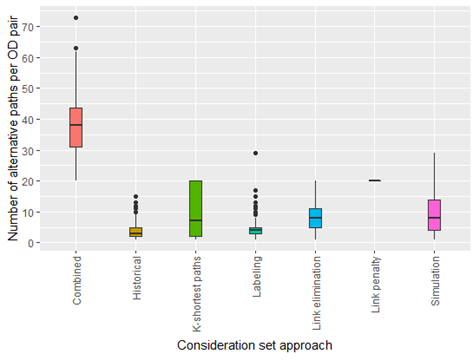
\includegraphics[width=250pt]{./imagenes/sizecs.png}}
    \caption{Distribution of alternative paths per consideration set approach}
    \label{fig:distribution}
\end{figure}

For each consideration set approach, we calculated the average of each attribute that characterized the alternatives for each OD pair. In Table \ref{tab:statistics}, we show the mean and standard deviation of the average of path attributes for each generated consideration set approach. We use the Path Size (PS) Term presented in Equation (7) to evaluate the capacity of each approach to generate diverse paths. A PS term equal to zero means that the generated alternative paths included in the consideration set are not overlapped (the alternatives are all different). A more negative PS term means that the generated alternative paths included in the consideration set have a higher degree of overlap (the alternatives are more similar). The results in Table \ref{tab:statistics} show that the Combined approach generated the highest degree of overlap between alternatives. This is because, since the Combined approach includes more alternatives, there is a higher probability that they share links. Without considering the Combined approach, the Simulation and Link penalty approaches generate the most heavily overlapped alternative paths, while the Historical/Cohort, Labeling, and Link elimination approaches generate the most diverse alternative paths. 

Analyzing the number of transfers for each approach, the Historical/Cohort approach generates the fewest transfers on average, followed by the K-shortest path approach. Therefore, the K-shortest path approach generates fewer irrelevant path alternatives, on average, than the other heuristic approaches. The waiting time shows similar results, where the waiting times generated by the K-shortest path approach are quite similar to those of the Historical/Cohort approach. The Labeling approach generates paths with longer waiting times and walking transfer times, on average. This is expected, since the Labeling approach applies some labels that do not take waiting and walking transfer times into consideration. Regarding in-vehicle travel time, the K-shortest path approach and the Simulation approach obtained the results closest to the Historical/Cohort approach, while the Link penalty approach produced routes with the longest in-vehicle travel times.

\begin{table}[H]
\centering
% table caption is above the table
\footnotesize\setlength\tabcolsep{3 pt}
\caption{Statistics of alternatives path attributes for each consideration set approach}
\label{tab:statistics}  
\begin{tabular}{l|ll|ll|ll|ll|ll|ll}
\hline\noalign{\smallskip}
\multirow{2}{*}{\begin{tabular}[c]{@{}l@{}}Consideration set \\ approach\end{tabular}} & \multicolumn{2}{c|}{Size} & \multicolumn{2}{c|}{Path   Size} & \multicolumn{2}{c|}{\# of   transfers} & \multicolumn{2}{c|}{Waiting   time} & \multicolumn{2}{c|}{\begin{tabular}[c]{@{}l@{}}In-vehicle \\ travel time\end{tabular}} & \multicolumn{2}{c}{\begin{tabular}[c]{@{}l@{}}Walking time\\  in transfer\end{tabular}}  \\
                                            & Mean        & Std        & Mean            & Std           & Mean               & Std              & Mean             & Std             & Mean                  & Std                  & Mean                   & Std                   \\
\noalign{\smallskip}\hline\noalign{\smallskip}
Historical                                  & 3.8         & 2.5        & -1.2            & 0.7           & 0.8                & 0.9              & 7.7              & 3.3             & 25.5                  & 13.4                 & 1.0                    & 1.4                   \\
K-shortest paths                            & 10.0        & 7.7        & -2.2            & 1.1           & 1.2                & 0.7              & 8.5              & 3.0             & 24.4                  & 13.1                 & 0.6                    & 0.7                   \\
Labeling                                    & 4.2         & 2.8        & -1.7            & 0.7           & 2.4                & 2.1              & 22.8             & 24.2            & 27.2                  & 17.0                 & 1.2                    & 1.4                   \\
Link elimination                            & 8.7         & 4.5        & -1.7            & 0.6           & 1.5                & 0.9              & 14.1             & 12.0            & 29.1                  & 16.4                 & 1.1                    & 0.8                   \\
Link penalty                                & 20          & 0          & -2.6            & 0.4           & 1.7                & 0.7              & 12.4             & 3.3             & 29.9                  & 15.1                 & 1.1                    & 0.6                   \\
Simulation                                  & 9.5         & 6.4        & -2.3            & 1.0           & 2.1                & 1.7              & 14.5             & 7.9             & 25.6                  & 14.6                 & 1.1                    & 0.7                   \\
Combined                                    & 38.0        & 9.1        & -3.4            & 0.5           & 2.1                & 0.9              & 15.7             & 5.7             & 29.4                  & 15.3                 & 1.2                    & 1.1        \\    
\noalign{\smallskip}\hline
\end{tabular}
\end{table}

\subsection{Route choice models}

MNL models and PS logit models were estimated using a sample of 15,594 observations, which correspond to trips taken during the 15 business days comprising the first three weeks of data. Both types of logit models were estimated using the  Historical/Cohort, K-shortest paths, Labeling, Link elimination, Link penalty, Simulation, and Combined approaches. 

The specification of the deterministic utility function considers in-vehicle travel time, waiting time at the beginning of the trip and during transfers, walking time during transfers, and the transfer penalty, which considers bus-to-bus, bus-to-Metro, and Metro-to-bus transfers. Metro-to-Metro transfers cannot be incorporated into the model because the route that the passenger uses inside the Metro network cannot be observed from the data. 

Table \ref{tab:mnlmodel} shows the estimated parameters for the MNL logit models for each consideration set generation approach. The model that uses the Historical/Cohort reported parameters that are all are statistically significant (at the accepted 5\% threshold) with the expected sign. These results are similar to the models that use a heuristic approach (Labeling, Link elimination, Link penalty, Simulation, K-shortest paths, and Combined approaches), where the parameters are statistically significant and with the expected sign, with the exception of the transfer walking time parameter, which had a positive sign for all six heuristic approaches. 

Table \ref{tab:pslmodel} show the estimated parameters for the PS logit models for each consideration set generation approach. The PSC term is statistically significant in all models. Given that PSC lies within the interval (-∞,0] and implies a reduction in the systematic utility of correlated routes, the positive sign in the coefficient obtained for all models is expected. All models maintain the results shown in Table \ref{tab:mnlmodel}, in terms of statistical significance and the sign of the parameters.

Comparing the results of the MNL models and the PS logit models, the PS logit models present better model fit in all cases. Consequently, the inclusion of the PSC term in the specification of the models allows for greater explanatory power compared to the MNL models. In summary, these results show that, if correlation due to the overlapping between alternatives is considered in the model, all consideration set approaches can represent the perception of passengers with respect to the alternative path attributes, except for the transfer walking time attribute, which obtained an unexpected sign for heuristic approaches.

\section{Discussion}

This section analyzes the PS logit model parameters to understand the differences between each evaluated consideration set approach. 

The negative coefficients of the travel time and waiting time variables show a disutility of travel time for passengers. All models indicate that alternative routes with shorter in-vehicle travel time and waiting times are preferred. In the models, we estimated sensitivity to waiting time at the beginning of the trip as well as at any transfer stages. Table \ref{tab:ratessub} shows that the results of the rates of substitution of initial waiting time with respect to in-vehicle travel time vary between 1 and 1.4. Focusing on transfer waiting time, the rates of substitution obtained with most of the consideration set approaches are around 2, which is in line with the public transport route choice literature \citep{nassir2018strategy, rui2016modeling, raveau2014analyzing}. However, the Link elimination approach and the K-shortest paths approach generate a rate of substitution of transfer waiting time value close to 3. 

The disutility of the walking transfer time variable can only be represented by the model that uses the Historical/Cohort approach, which generates a rate of substitution of around 1.2 (see Table \ref{tab:ratessub}). This attribute cannot be evaluated for the other approaches, since their models generate a positive parameter. The trade-offs between in-vehicle travel time and transfer walking time obtained with the Historical/Cohort approach are in line with some studies that have reported a value between 1 and 2 \citep{janovsikova2014estimation, nassir2018strategy}. \citep{raveau2014analyzing} reported a value of around 3 minutes for this trade-off; the model that uses the Historical/Cohort approach is closest to this value. 

The negative coefficient of the transfer variable shows a disutility of the number of transfers for passengers. All models indicate that passengers prefer alternative routes with the lowest number of transfers. As shown in Table \ref{tab:ratessub}, the results of the rates of substitution of the number of transfers with respect to in-vehicle travel time vary between 13 and 54 minutes. The smallest value is reported by the model that uses the Historical/Cohort approach and the highest value is reported by the model that uses the Simulation approach. Previous studies have shown that one transfer is perceived by a typical passenger as equivalent to a number that varies between 3.6 min and 16 min of in-vehicle time \citep{guo2011assessing, nassir2018strategy, raveau2014analyzing, rui2016modeling}. Therefore, the model that uses the Historical/Cohort approach seems to best represent the perception of passengers regarding transfers.

For a prediction analysis, the trip dataset is split into two parts. The parameters obtained from the estimation are used to predict the paths chosen in the second part of the dataset, which corresponds to 4,685 weekday observations from the fourth week of data. We use the First Preference Recovery (FPR) and the Average Loglikelihood (AL) to evaluate the performance of each consideration set approach. Table \ref{tab:prediction} shows the FPR and AL values for the models constructed with each consideration set approach. The Historical/Cohort approach resulted in the best prediction performance.

In summary, the results of this study suggest that the Historical/Cohort approach obtained the highest level of prediction accuracy, and it is the only approach that returns, for all attributes evaluated in this study, similar rates of substitution reported in the public transport route choice modelling literature.

\begin{landscape}
\begin{table}[]
\centering
% table caption is above the table
\footnotesize\setlength\tabcolsep{3 pt}
\caption{MNL model estimates (t tests) using each generation consideration set approach}
\label{tab:mnlmodel}  
\begin{tabular}{llllllll}
\hline\noalign{\smallskip}
\multicolumn{1}{c}{\multirow{2}{*}{Parameters}} & \multicolumn{7}{c}{Consideration set approach}                                                                              \\
\multicolumn{1}{c}{}                            & Historical/Cohort & Simulation     & Labeling       & Link penalty   & Link elimination & K-shortest paths & Combined       \\
\noalign{\smallskip}\hline\noalign{\smallskip}
Travel time in vehicle                          & -0.144 (-47.3)    & -0.082 (-24.1) & -0.181 (-58)   & -0.197 (-74.9) & -0.145 (-55.6)   & -0.113 (-34.3)   & -0.184 (-78.2) \\
Initial waiting time                            & -0.162 (-39.5)    & -0.036 (-7)    & -0.116 (-25.1) & -0.192 (-42.6) & -0.152 (-33.2)   & -0.073 (-15.2)   & -0.19 (-43.1)  \\
Transfer waiting time                           & -0.304 (-23.5)    & -0.269 (-22.5) & -0.196 (-12.8) & -0.434 (-33.4) & -0.383 (-28.5)   & -0.395 (-22.3)   & -0.29 (-30.6)  \\
Transfer walking time                           & -0.152 (-12.8)    & 1.081 (38)     & 1.101 (37.3)   & 1.209 (54.2)   & 1.294 (42.1)     & 1.557 (49.4)     & 0.961 (45.9)   \\
Transfer                                        & -1.374 (-16.3)    & -3.77 (-39.9)  & -3.463 (-33)   & -5.285 (-61.2) & -4.364 (-45.3)   & -5.167 (-49.7)   & -5.757 (-72.3) \\
\# of observations                              & 15,594            & 15594          & 15594          & 15594          & 15594            & 15594            & 15594          \\
Log-likelihood                                  & -16736.7          & -11493.8       & -12943.4       & -16497.0       & -14467.9         & -13525.8         & -17695.9       \\
Adjusted rho-square                             & 0.123             & 0.61           & 0.40           & 0.65           & 0.55             & 0.57             & 0.68           \\
AIC                                             & 33483.3           & 22997.7        & 25896.8        & 33003.9        & 28945.8          & 27061.6          & 35488.3     \\
\noalign{\smallskip}\hline
\end{tabular}
\vskip 0.05cm
%\centering
\footnotesize{All columns show t-values between parentheses. AIC = Akaike information criterion.}
\end{table}

\begin{table}[]
\centering
% table caption is above the table
\footnotesize\setlength\tabcolsep{3 pt}
\caption{PS Logit model estimates (t tests) using each generation consideration set approach}
\label{tab:pslmodel}  
\begin{tabular}{llllllll}
\hline\noalign{\smallskip}
\multicolumn{1}{c}{\multirow{2}{*}{Parameters}} & \multicolumn{7}{c}{Consideration set approach}                                                                              \\
\multicolumn{1}{c}{}                            & Historical/Cohort & Simulation     & Labeling       & Link penalty   & Link elimination & K-shortest paths & Combined       \\
\noalign{\smallskip}\hline\noalign{\smallskip}
Travel time in vehicle      & -0.119 (-37.7)    & -0.096 (-21.5) & -0.129 (-32.9)       & -0.173 (-62.3) & -0.111 (-36)     & -0.135 (-37)     & -0.181 (-72.9) \\
Initial waiting time        & -0.131 (-30.7)    & -0.137 (-20.6) & -0.147 (-25.8)       & -0.193 (-40.3) & -0.144 (-28.7)   & -0.132 (-25.7)   & -0.236 (-52.2) \\
Transfer waiting time       & -0.257 (-18.7)    & -0.181 (-12.6) & -0.205 (-10)         & -0.366 (-26.3) & -0.32 (-22.8)    & -0.393 (-19.4)   & -0.262 (-26.7) \\
Transfer walking time       & -0.144 (-12.1)    & 0.478 (8.7)    & 0.624 (13.4)         & 0.693 (22.5)   & 0.924 (24.6)     & 1.323 (38.1)     & 0.596 (22)     \\
Transfer                    & -1.527 (-18)      & -5.177 (-32.2) & -4.118 (-26.6)       & -5.155 (-49)   & -4.261 (-42.4)   & -5.128 (-43.6)   & -5.846 (-63.7) \\
PSC                         & 1.085 (29.5)      & 1.753 (46.2)   & 1.841 (57)           & 1.274 (50.4)   & 1.234 (55.9)     & 0.735 (32.5)     & 0.834 (43.6)   \\
\# of observations          & 15,594            & 15594          & 15594                & 15594          & 15594            & 15594            & 15594          \\
Log-likelihood              & -16180.1          & -8086.6        & -9707.4              & -15066.4       & -12739.4         & -13133.1         & -16736.2       \\
Adjusted rho-square         & 0.152             & 0.73           & 0.55                 & 0.68           & 0.60             & 0.58             & 0.70           \\
AIC                         & 32372.1           & 16185.3        & 19426.9              & 30144.9        & 25490.8          & 26278.2          & 33484.5    \\
\noalign{\smallskip}\hline
\end{tabular}
\vskip 0.05cm
\footnotesize{All columns show t-values between parentheses. AIC = Akaike information criterion.}
\end{table}

\begin{table}[]
\centering
% table caption is above the table
\footnotesize\setlength\tabcolsep{3 pt}
\caption{Rates of substitution of parameters obtained with the PS Logit model using each generation consideration set approach}
\label{tab:ratessub}  
\begin{tabular}{lccccccc}
\hline\noalign{\smallskip}
\multirow{2}{*}{Parameters} & \multicolumn{7}{c}{Consideration set approach}                                                            \\
                            & Historical/Cohort & Simulation & Labeling & Link penalty & Link elimination & K-shortest paths & Combined \\
\noalign{\smallskip}\hline\noalign{\smallskip}
Travel time in vehicle      & 1.00              & 1.00       & 1.00     & 1.00         & 1.00             & 1.00             & 1.00     \\
Initial waiting time        & 1.10              & 1.43       & 1.14     & 1.11         & 1.30             & 0.98             & 1.31     \\
Transfer waiting time       & 2.16              & 1.88       & 1.59     & 2.11         & 2.90             & 2.91             & 1.45     \\
Transfer walking time       & 1.21              & -4.98      & -4.85    & -4.00        & -8.36            & -9.80            & -3.30    \\
Transfer                    & 12.86             & 53.93      & 32.01    & 29.77        & 38.53            & 37.99            & 32.38   \\
\noalign{\smallskip}\hline
\end{tabular}
\end{table}

\begin{table}[]
\centering
% table caption is above the table
\footnotesize\setlength\tabcolsep{3 pt}
\caption{Prediction results}
\label{tab:prediction} 
\begin{tabular}{lccccccc}
\hline\noalign{\smallskip}
\multicolumn{1}{c}{\multirow{2}{*}{Indicator}} & \multicolumn{7}{c}{Consideration set approach}                                                            \\
\multicolumn{1}{c}{}                            & Historical/Cohort & Simulation & Labeling & Link penalty & Link elimination & K-shortest paths & Combined \\
\noalign{\smallskip}\hline\noalign{\smallskip}
First preference recovery                       & 0.5266            & 0.4603     & 0.5057   & 0.4827       & 0.4941           & 0.4556           & 0.4954   \\
Loglikelihood of validation sample              & 0.4451            & 0.2572     & 0.3500   & 0.3692       & 0.3569           & 0.3433           & 0.3476  \\
\noalign{\smallskip}\hline
\end{tabular}
\end{table}

\end{landscape}

\section{Conclusions}

Modeling route choice behavior requires the identification of non-chosen paths considered attractive by travelers to reach a destination. This set of alternatives is call the consideration set and is usually unknown to researchers working with revealed preference data. Most public transport route choice studies that work with this type of data have identified the consideration set through ad-hoc heuristics, such as shortest path algorithms \citep{rui2016modeling} or using historical data \citep{janovsikova2014estimation, kim2019calibration}. We use a variation of the historical data approach, which we term the Historical/Cohort approach, to impute the past observed choices made by the traveler, or by other users in the same cohort in cross section data, as the consideration set. In this study, we first present the theoretical conditions under which the Historical/Cohort approach would recover the population parameters. We then use a case study to assess the performance of different consideration set generation approaches, which are commonly used in the transport route choice literature, in terms of estimation and prediction. The results show that the Historical/Cohort approach surpasses the other methods with regards to all statistics considered.

The proof of the Historical/Cohort approach is based on an adaptation of the theorem of sampling of alternatives \citep{mcfadden1978}, in which prior choices are understood as draws from the true consideration set, and the sampling correction cancels out when there are many observations and invariability conditions hold. In this context, we hypothesize that route choice models that use the Historical/Cohort approach to identify the consideration set obtain the same or better results than any other consideration set generation approach. 

To evaluate this research hypothesis, we use data from the public transport system in Santiago, Chile to estimate route choice models with different consideration set generation approaches: the Historical/Cohort approach and six approaches based on shortest path heuristics: the Labeling, Link elimination, Link penalty, K-shortest paths, Simulation, and Combination (of all prior) approaches. To do so, we split the database in two parts, the first corresponding to three weeks of weekday data and the second corresponding to weekday data from the fourth week. Using the first part of the database, we estimated two RUM models using each consideration set generation approach: a MNL model, which is the basic and most used model to represent route choice in public transport systems, and a PS logit model, which captures correlation due to overlapping between alternative paths. The results show that all PS logit models obtained a better fit than the MNL models. Focusing on the PS logit models, the estimated parameters suggest that all consideration set generation approaches can well-represent the perception of passengers for all attributes, except for the transfer walking time, which is well-represented only by the Historical/Cohort approach. Regarding the rates of substitution with respect to in-vehicle travel time, the Historical/Cohort approach is the only model that returns values previously reported in the public transport literature for all attributes. The only attribute for which all consideration set generation approaches returned a rate of substitution reported in previous studies was the initial waiting time. For other attributes, one or more heuristic approaches reported non-expected values. The evidence from this analysis supports the idea that the Historical/Cohort approach to identify the consideration set accurately estimates the population parameters. In addition, the comparison of prediction accuracy across different consideration set generation approaches suggests that the Cohort/Historical approach estimates models with better predictive abilities with respect to the choices of passengers in the prediction sample. 


\bibliographystyle{apacite}
\bibliography{sample}

\end{document}